
\documentclass[submit]{harvardml}

% Put in your full name and email address.
\name{Luke Mueller}
\email{lam908@mail.harvard.edu}

% List any people you worked with.
\collaborators{%
}

% You don't need to change these.
\course{CS181-S16}
\assignment{Assignment \#3}
\duedate{5:00pm March 25, 2016}

\usepackage[OT1]{fontenc}
\usepackage[colorlinks,citecolor=blue,urlcolor=blue]{hyperref}
\usepackage[pdftex]{graphicx}
\usepackage{subfig}
\usepackage{fullpage}
\usepackage{palatino}
\usepackage{mathpazo}
\usepackage{amsmath}
\usepackage{amssymb}
\usepackage{color}
\usepackage{todonotes}
\usepackage{listings}
\usepackage{common}
\usepackage{bm}

\usepackage[mmddyyyy,hhmmss]{datetime}

\definecolor{verbgray}{gray}{0.9}

\lstnewenvironment{csv}{%
  \lstset{backgroundcolor=\color{verbgray},
  frame=single,
  framerule=0pt,
  basicstyle=\ttfamily,
  columns=fullflexible}}{}

\begin{document}
\begin{center}
{\Large Homework 3: SVM}\\
\end{center}

There is a mathematical component and a programming component to this homework.
Please submit ONLY your PDF to Canvas, and push all of your work to your Github
repository. If a question asks you to make any plots, like Problem 3, please
include those in the writeup.

%%%%%%%%%%%%%%%%%%%%%%%%%%%%%%%%%%%%%%%%%%%%%
% Problem 1
%%%%%%%%%%%%%%%%%%%%%%%%%%%%%%%%%%%%%%%%%%%%%
\begin{problem}[Fitting an SVM by hand, 8pts]
Consider a dataset with the following 6 points in $1D$: \[\{(x_1, y_1)\} =\{(-3
, +1 ), (-2 , +1 ) , (-1,  -1 ), ( 1 , -1 ), ( 2 , +1 ), ( 3 , +1 )\}\] Consider
mapping these points to $2$ dimensions using the feature vector $\phi : x
\mapsto (x, x^2)$. The max-margin classifier objective is given by:
\begin{equation}
  \min_{\mathbf{w}, w_0} \|\mathbf{w}\|_2^2 \quad \text{s.t.} \quad y_i(\mathbf{w}^T \phi(x_i) +
  w_0) \geq 1,~\forall i
\end{equation}

Note: the purpose of this exercise is to solve the SVM without the help of a
computer, relying instead on principled rules and properties of these
classifiers. The exercise has been broken down into a series of questions, each
providing a part of the solution. Make sure to follow the logical structure of
the exercise when composing your answer and to justify each step.

\begin{enumerate}
  \item Write down a vector that is parallel to the optimal vector $\mathbf{w}$. Justify
    your answer.
  \item What is the value of the margin achieved by $\mathbf{w}$? Justify your
    answer.
  \item Solve for $\mathbf{w}$ using your answers to the two previous questions.
  \item Solve for $w_0$. Justify your answer.
  \item Write down the discriminant as an explicit function of $x$.
\end{enumerate}

\end{problem}
\subsection*{Solution}

\begin{enumerate}
	\item First, we note that $\mathbf{w}$ is orthogonal to the decision boundary given by $y_i(\mathbf{w}^T \phi(x_i) +
	w_0)=0$ since for two points $x_1$ and $x_2$ on the decision boundary, $(x_1-x_2)*\mathbf{w} = -w_0-(-w_0) = 0$. Then, considering $x_\perp$, which is defined as the vector on the decision boundary to satisfy the equation $\phi(x_\perp)+r\frac{\mathbf{w}}{||\mathbf{w}||_2}=\phi(x_i)$ for some point $\phi(x_i)$ in our data, we know that $\phi(x_i)-\phi(x_\perp)$ will also be orthogonal to the decision boundary. Thus, it follows that $\mathbf{w} \parallel \phi(x_i)-\phi(x_\perp)$. \\\\
	For example, taking the point $\phi(x_i) = ((2,4),+1)$ whose respective $\phi(x_\perp) = ((2,2.5),0)$:
	\[
	\mathbf{w} \parallel \phi(x_i)-\phi(x_\perp) = ((2,4),+1)-((2,2.5)0) = (0,1.5)
	\]
	
	\item The value of the margin achieved by $\mathbf{w}$ is easily seen in a $2D$ diagram of $\phi(x)$, since the support vectors are made obvious. In particular, for $y_2=+1$ the support vectors are $((-2,4),+1)$ and $((2,4),+1)$ and for $y_2=-1$ the support vectors are $((-1,1),-1)$ and $((1,1),-1)$. We know this because $(1)$: they are the closest, oppositely classified vectors in the data, and $(2)$: the difference between these positively classified vectors is parallel to the difference in these negatively classified vectors, and thus, also parallel to the optimal decision boundary. Then, placing the decision boundary equidistant from these $4$ support vectors, we can calculate the margin achieved by $\mathbf{w}$ as the distance between any support vector and the decision boundary, which comes out to $1.5$.
	
	\item To determine $\mathbf{w}$, we make use of the following:
	\begin{align*}
	& \phi(x_\perp)+r\frac{\mathbf{w}}{||\mathbf{w}||_2}=\phi(x_i) \\
	& r = \frac{1}{||\mathbf{w}||_2}(\phi(x)\mathbf{w}^T+w_o) \\
	& r=1.5 &
	\end{align*}
	
	The first equation we defined previously. The second is the geometric margin, and we make use of the fact that $\mathbf{w}$ is determined when the functional margin $(\phi(x)\mathbf{w}^T+w_o) $ equals $1$. The third equation is given by the solution to $(2.)$ Thus we have:
	
	\begin{align*}
	\phi(x_\perp)+r\frac{\mathbf{w}}{||\mathbf{w}||_2}=\phi(x_i) \Rightarrow \frac{\mathbf{w}}{||\mathbf{w}||_2} & = \frac{\phi(x_i)-\phi(x_\perp)}{r} \\
	& = \frac{(2,4)-(2,2.5)}{1.5} = \frac{(0,1.5)}{1.5} &
	\end{align*}
	
	Then solving for $||\mathbf{w}||_2$:
	
	\begin{align*}
	r = \frac{1}{||\mathbf{w}||_2}(\phi(x)\mathbf{w}^T+w_o) = \frac{1}{||\mathbf{w}||_2} \Rightarrow ||\mathbf{w}||_2 & = \frac{1}{r} \\
	& = \frac{1}{1.5} = 2/3
	\end{align*}
	
	Then solving for $\mathbf{w}$
	
	\begin{align*}
	\mathbf{w} & = \frac{\phi(x_i)-\phi(x_\perp)}{r} \times ||\mathbf{w}||_2 \\
	& = \frac{(0,1.5)}{(1.5)^2} = (0, 2/3)^T
	\end{align*}
	
	\item To solve for $w_0$ we input $\mathbf{w}$ and some point $\phi(x_i)$ into the functional margin. In particular we have:
	
	\[
	(\phi(x)\mathbf{w}^T+w_o) = 1 \Rightarrow w_0 = 1 - \phi(x)\mathbf{w}^T = 1 - (2,4)\cdot(0,2/3) = 1 - (0 + 8/3) = -1 \frac{2}{3}
	\]
	
	\item Using values for $\mathbf{w}$ and $w_0$ we write the discriminant as an explicit function of $x$:
	
	\begin{equation}
	y_i = \mathbf{w}^T\phi(x_i)+w_0 = (0,\frac{2}{3})^T\cdot(x_i,x_i^2) - 1\frac{2}{3}
	\end{equation}
\end{enumerate}


\newpage
%%%%%%%%%%%%%%%%%%%%%%%%%%%%%%%%%%%%%%%%%%%%%
% Problem 2
%%%%%%%%%%%%%%%%%%%%%%%%%%%%%%%%%%%%%%%%%%%%%
\begin{problem}[Composing Kernel Functions , 7pts]
Prove that
\begin{align*}
	K(\boldx, \boldx') &= \exp\{ -||\boldx - \boldx'||^2_2 \}\,,
\end{align*}
where~$\boldx,\boldx'\in\reals^D$ is a valid kernel, using only the following
properties.  If~$K_1(\cdot,\cdot)$ and~$K_2(\cdot,\cdot)$ are valid kernels,
then the following are also valid kernels:
\begin{align*}
	(1) \quad K(\boldx, \boldx') &= c\,K_1(\boldx, \boldx') \quad \text{for $c>0$}\\
	(2) \quad K(\boldx, \boldx') &= K_1(\boldx, \boldx') + K_2(\boldx, \boldx')\\
	(3) \quad K(\boldx, \boldx') &= K_1(\boldx, \boldx')\,K_2(\boldx, \boldx')\\
	(4) \quad K(\boldx, \boldx') &= \exp\{ K_1(\boldx, \boldx') \}\\
    (5) \quad K(\boldx, \boldx') &= f(\boldx)\,K_1(\boldx, \boldx')\,f(\boldx') \quad
  \text{where $f$ is any function from~$\reals^D$ to $\reals$}
\end{align*}

 \end{problem}
\subsection*{Solution}

First, we expand the square $||\mathbf{X}-\mathbf{X}'||_2^2$ as in Bishop $6.24$ to get:
\[
\mathbf{X}^T\mathbf{X}+(\mathbf{X}')^T\mathbf{X}'-2\mathbf{X}^T\mathbf{X}'
\]

\noindent
Then multiplying by $-1$ and exponentiating we obtain:
\[
\exp\{-\mathbf{X}^T\mathbf{X}\}\exp\{2\mathbf{X}^T\mathbf{X}'\}\exp\{-(\mathbf{X}')^T\mathbf{X}'\}
\]

\noindent
Which is a valid kernel due to:
\begin{enumerate}
	\item The validity of the linear kernel $k(\mathbf{X},\mathbf{X'})=\mathbf{X}^T\mathbf{X}$, which is present in all 3 terms.
	\item The validity of a kernel multiplied by a scalar to account for the $2$ in the second term
	\item The validity of the exponent of a valid kernel, given by (4) above, which applies to all 3 terms.
	\item The validity of a kernel in the form given by (5) above, where the first and third terms are a function of $\mathbf{X}$ and the second term, $\exp\{2\mathbf{X}^T\mathbf{X}'\}$, is equivalent to $K_1(\boldx, \boldx')$ in (5).
\end{enumerate}

\newpage
%%%%%%%%%%%%%%%%%%%%%%%%%%%%%%%%%%%%%%%%%%%%%
% Problem 3
%%%%%%%%%%%%%%%%%%%%%%%%%%%%%%%%%%%%%%%%%%%%%
\begin{problem}[Scaling up your SVM solver, 10pts (+7pts with extra credit)]



In the previous homework, you studied a simple data set of fruit measurements.
We would like you to code up a few simple SVM solvers to classify lemons from
apples. To do this, read the paper at
\url{http://www.jmlr.org/papers/volume6/bordes05a/bordes05a.pdf} and implement
the Kernel Perceptron algorithm and the Budget Kernel Perceptron algorithm. The provided code has a base Perceptron class, which you will inherit to write KernelPerceptron and BudgetKernelPerceptron. This has been set up for you in problem3.py. The provided data is linearly separable. Make the optimization as fast as
possible. 

Additionally, we would like you to do some experimentation with the hyperparameters for each of these models. Try seeing if you can identify some patterns by changing $\beta$, N (maximum number of support vectors), or the number of random samples you take.  Note the training time, accuracy,  shapes/orientations of hyperplanes, and number of support vectors for various setups. We are intentionally leaving this open-ended to allow for experimentation, and so we will be looking for your thought process and not a rigid graph this time. That being said, any visualizations that you want us to grade and refer to in your descriptions should be included in this writeup. You can use the trivial $K(\mathbf{x_1}, \mathbf{x_2}) = \mathbf{x_1}^T\mathbf{x_2}$ kernel for this problem, though you are welcome to experiment with more interesting kernels too. Also, answer the following reading questions in one or two sentences each.

\begin{enumerate}
\item In one short sentence, state the main purpose of the paper?
\item Identify each of the parameters in Eq. 1
\item State one guarantee for the Kernel perceptron algorithm described in the
  paper.
\item What is the main way the budget kernel perceptron algorithm tries to
  improve on the perceptron algorithm.
\item In simple words, what is the theoretical guarantee of LASVM algorithm? How
  does it compare to its practical performance?
\end{enumerate}


For extra credit (+7 pts), implement the SMO algorithm and implement the LASVM process and do the same as above.




\end{problem}

\subsection*{Solution}

\begin{enumerate}
	\item The main purpose of the paper is to explore properties of various kernel classifiers in order to determine whether certain "examples" in our data should be given additional computing time.
	
	\item Eq. 1: $\hat{y}(x)=w'\boldsymbol{\phi}(x)+b$
	\begin{itemize}
		\item $\hat{y}(x)$ is the predicted classification for input value $x$.
		\item $w'$ is a parameter vector that maps input x onto its predicted classification.
		\item $\boldsymbol{\phi}(x)$ is the feature vector transforming $x$.
		\item $b$ is the bias parameter that displaces $w'\boldsymbol{\phi}(x)$ from the origin.
	\end{itemize}
	
	\item One guarantee of the Kernel perceptron algorithm described in the paper is "When a solution exists, Novikoff’s Theorem (Novikoff, 1962) states that the algorithm converges after a finite number of mistakes, or equivalently after inserting a finite number of support vectors".
	
	\item The budget kernel perceptron algorithm attempts to improve on the perceptron algorithm by adding a step to remove support vectors from the kernel expansion, thus setting an upper bound to the number of support vectors generated by the algorithm. In particular, it introduces a hyperparameter $\beta$ instead of $0$ for the condition $y_t\hat{y}(x_t)\leq\beta$, and adds an additional condition, "If $|S| > N$ then $S \leftarrow S - \{\arg\max_{i\epsilon S} y_i (\hat{y}(x_i)-\alpha_i K(x_i, x_i))\}$".
	
	\item The theoretical guarantee of the LASVM algorithm is that it converges to the solution of the SVM QP (Quadratic Programming) problem after sufficient sequential passes over the training examples. However, experimental evidence indicates that LASVM matches the SVM accuracy after a single sequential pass over the training examples (page 1585). In other words, if we run the LASVM algorithm enough times we will arrive at the SVM solution, but practically speaking, we only need to run LASVM once to get a sufficient solution.
	
\end{enumerate}

\newpage

\subsection*{Problem 3 Results}

\begin{table}[htb]
	\centering
	\caption{Hyperparameter Tuning}
	\label{my-label}
	\begin{tabular}{lcccccc}
		\textbf{Model} & \textbf{Beta}                & \textbf{N}                 & \textbf{Numsamples}          & \textbf{\# Support Vectors} & \textbf{Process Time (s)} & \textbf{Accuracy}    \\
		& \multicolumn{1}{l}{}         & \multicolumn{1}{l}{}       & \multicolumn{1}{l}{}         & \multicolumn{1}{l}{}        & \multicolumn{1}{l}{}  & \multicolumn{1}{l}{} \\
		model 1 k                            & 0                            & 100                        & 20000                        & 13                          & 0.98481               & 1                    \\
		model 1 bk                           & 0                            & 100                        & 20000                        & 100                         & 9.364486              & 0.9999392633         \\
		&                              &                            &                              &                             &                       &                      \\
		model 2 k                            & 0                            & {\color[HTML]{3166FF} 200} & 20000                        & 184                         & 6.807833              & 1                    \\
		model 2 k                            & 0                            & {\color[HTML]{3166FF} 200} & 20000                        & 200                         & 19.112219             & 1                    \\
		&                              &                            &                              &                             &                       &                      \\
		model 3 k                            & 0                            & {\color[HTML]{3166FF} 500} & 20000                        & 212                         & 8.086729              & 1                    \\
		model 3 bk                           & 0                            & {\color[HTML]{3166FF} 500} & 20000                        & 70                          & 6.900058              & 1                    \\
		&                              &                            &                              &                             &                       &                      \\
		model 4 k                            & 0                            & 100                        & {\color[HTML]{3531FF} 10000} & 158                         & 3.531878              & 0.9998785265         \\
		model 4 bk                           & 0                            & 100                        & {\color[HTML]{3531FF} 10000} & 100                         & 4.804197              & 0.9620395396         \\
		&                              &                            &                              &                             &                       &                      \\
		model 5 k                            & 0                            & 100                        & {\color[HTML]{3166FF} 30000} & 103                         & 8.50177               & 1                    \\
		model 5 bk                           & 0                            & 100                        & {\color[HTML]{3166FF} 30000} & 100                         & 15.577188             & 1                    \\
		&                              &                            &                              &                             &                       &                      \\
		model 6 k                            & 0                            & 100                        & {\color[HTML]{3166FF} 50000} & 200                         & 23.909554             & 1                    \\
		model 6 bk                           & 0                            & 100                        & {\color[HTML]{3166FF} 50000} & 99                          & 25.03202              & 0.9875793374         \\
		&                              &                            &                              &                             &                       &                      \\
		model 7 k                            & {\color[HTML]{3166FF} 0.5}   & 100                        & 20000                        & 87                          & 5.084028              & 1                    \\
		model 7 bk                           & {\color[HTML]{3166FF} 0.5}   & 100                        & 20000                        & 100                         & 10.82751              & 0.9806553494         \\
		&                              &                            &                              &                             &                       &                      \\
		model 8 k                            & {\color[HTML]{3166FF} 0.05}  & 100                        & 20000                        & 231                         & 8.934602              & 0.9999392633         \\
		model 8 bk                           & {\color[HTML]{3166FF} 0.05}  & 100                        & 20000                        & 100                         & 10.938737             & 0.9921345926         \\
		&                              &                            &                              &                             &                       &                      \\
		model 9 k                            & {\color[HTML]{3166FF} -0.05} & 100                        & 20000                        & 280                         & 9.548529              & 1                    \\
		model 9 bk                           & {\color[HTML]{3166FF} -0.05} & 100                        & 20000                        & 0                           & 0.268766              & 0                    \\
		&                              &                            &                              &                             &                       &                      \\
		model 10 k                           & {\color[HTML]{3166FF} 0.05}  & {\color[HTML]{3166FF} 200} & {\color[HTML]{3166FF} 10000} & 236                         & 4.174034              & 0.9856964985         \\
		model 10 bk                          & {\color[HTML]{3166FF} 0.05}  & {\color[HTML]{3166FF} 200} & {\color[HTML]{3166FF} 10000} & 200                         & 8.645547              & 0.9712411552         \\
		&                              &                            &                              &                             &                       &                      \\
		model 11 k                           & {\color[HTML]{3166FF} 0.05}  & {\color[HTML]{3166FF} 500} & {\color[HTML]{3166FF} 10000} & 138                         & 3.240456              & 0.9999392633         \\
		model 11 bk                          & {\color[HTML]{3166FF} 0.05}  & {\color[HTML]{3166FF} 500} & {\color[HTML]{3166FF} 10000} & 406                         & 11.599665             & 0.9861823924        
	\end{tabular}
\end{table}

Table 1 shows the relative performances of the Kernel Perceptron algorithm (k) and the Budget Kernel Perceptron algorithm (bk) under different hyperparameter values. In particular, we have:

\begin{itemize}
	\item $beta$: the missclassification condition
	\item $N$: the upper bound for support vectors. Applied only in Budget Kernel Perceptron
	\item $numsamples$: the number of examples taken from the training data to execute the algorithms. Applied only in Budget Kernel Perceptron
\end{itemize}

The process time is represented in seconds. The accuracy was determined by splitting the data into training and validation sets, fitting the training data with the algorithm, using the fit to predict new values for the validation data, and computing the proportion of correctly classified validation predictions.

In general, all models provided near perfect accuracy with varied process time across different values for the hyperparameters. As expected, increasing the number of samples provided the best accuracy with the greatest cost of process time. Increasing the upper bound for the support vectors also increased process time, but did not necessarily improve the accuracy. Changing beta decreased accuracy as it deviated further from 0.

Notably, though the accuracy metric reveals slight differences between models, relatively speaking there were no substantial differences. 

The Kernel Perceptron algorithm generally ran faster, and provided greater accuracy than the Budget Kernel Perceptron algorithm. Model 3 was an exception, where the upper bound on the number of support vectors was large. 

The shapes/orientations of the hyperplanes were slightly different under some hyperparameter settings, as seen in figures 1 and 2. They were identical however, when $numsamples$ was large - since the support vectors were not as dominated by the algorithms' random example selections. 

To summarize, the Kernel Perceptron algorithm generally performed better than the Budget Kernel Perceptron algorithm with regards to training process time and validation accuracy. This is likely due to the fact that our data are not very "noisy", thus the benefits provided by the Budget Kernel Perceptron algorithm are somewhat lost. Concretely, the increased margin provided by the modified decision boundary under the Budget Kernel Perceptron algorithm was unnecessary, and possibly even over-fitted while costing us additional computation time.




\begin{figure}[!tbp]
	\centering
	\begin{minipage}[b]{0.4\textwidth}
		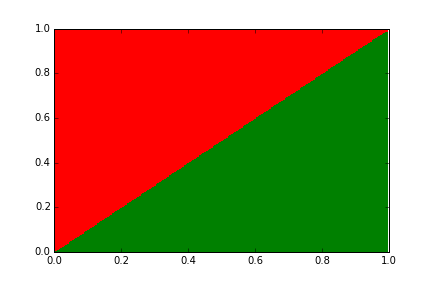
\includegraphics[width=\textwidth]{k.png}
		\caption{Kernel Perceptron.}
	\end{minipage}
	\hfill
	\begin{minipage}[b]{0.4\textwidth}
		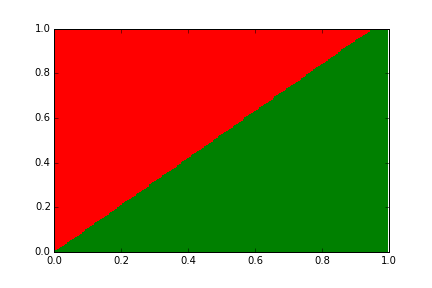
\includegraphics[width=\textwidth]{bk.png}
		\caption{Budget Kernel Perceptron.}
	\end{minipage}
\end{figure}


\newpage

\subsection*{Calibration [1pt]}
Approximately how long did this homework take you to complete? \\
15 hours.


\end{document}


















































